\documentclass{article}
\usepackage{arxiv}

\usepackage[utf8]{inputenc}
\usepackage[english]{babel}
\usepackage[T1]{fontenc}
\usepackage{url}
\usepackage{booktabs}
\usepackage{amsfonts}
\usepackage{nicefrac}
\usepackage{microtype}
\usepackage{lipsum}
\usepackage{graphicx}
\usepackage{natbib}
\usepackage{doi}
\usepackage[colorinlistoftodos]{todonotes}
\usepackage{hyperref}

\renewcommand{\headeright}{Draft}
\renewcommand{\undertitle}{Draft}

\title{Winterstorm Prediction via Deep Learning}

\author{ Kornilov Nikita\\
	Department of Control and Applied Mathematics\\
	Moscow Institute of Physics and Technology\\
	\texttt{kornilov.nm@phystech.edu} \\
	\texttt{\href{https://colab.research.google.com/drive/1HBB8002s5_tFgFxGzIZQcBmsOsW6YcMh?usp=sharing} {Project code}}
	%% \AND
	%% Coauthor \\
	%% Affiliation \\
	%% Address \\
	%% \texttt{email} \\
	%% \And
	%% Coauthor \\
	%% Affiliation \\
	%% Address \\
	%% \texttt{email} \\
	%% \And
	%% Coauthor \\
	%% Affiliation \\
	%% Address \\
	%% \texttt{email} \\
}
\date{}

\renewcommand{\shorttitle}{Winterstorms}

%%% Add PDF metadata to help others organize their library
%%% Once the PDF is generated, you can check the metadata with
%%% $ pdfinfo template.pdf
\hypersetup{
pdftitle={A template for the arxiv style},
pdfsubject={q-bio.NC, q-bio.QM},
pdfauthor={Kornilov Nikita},
pdfkeywords={Maximum risk prediction},
}

\begin{document}
\maketitle

\begin{abstract}
	In article problem of  harsh winterstorm prediction in short-term period is observed. This prediction is computed in large spacial grid. For practical needs model must accurately predict extreme events meanwhile on ordinary events it can make big number of mistakes.
\end{abstract}


\keywords{Maximum risk prediction, GRU-CNN models, extreme events theory }

\section{Introduction}
Extreme natural events such as winterstorms are serious and relevant problem for every country. Having information about upcoming events, companies can better prepare, survive and recover much faster after it. 

Researches in this area are attempting to predict location and time of future harsh natural event using climate data that was collected during last decades.\cite{EVL:1,LSTMCNN:2, GRUCNN:3} Especially, most dangerous and rare events are called extreme. Their prediction is much harder because of lack of information and unique patterns.
Traditional methods such as autoregressive moving average (ARMA) and nonlinear autoregressive exogenous (NARX) use statistical models with few parameters to exploit
patterns in time series data. But recently number of methods using Deep Learning approaches has greatly increased.  

In work \cite{LSTMCNN:2} was proposed method to predict events in spacial grid using combination of LSTM and CNN  neural networks architectures. Then, work \cite{EVL:1} showed progress in extreme events prediction proposing new models and loss functions based on extreme events theory that considered unique features of .

The current goal is to build model for short-term (up  to 20 years) prediction of winterstorms in North America using geodata from 1991 year about snow storms in this region. The data is partially very noised and inaccurate with spacial grid. 

In this article we expand extreme events prediction adding important spacial components to up-to-date methods. Also we use geographical area features. We combine together Recurrent Neural Networks architectures with CNN and state-of-the-art models for extreme events prediction.

Goal of research is to fit model with comparable quality to models from related works, that after can be used for other regions.
 
\section{Problem statement}
The extreme events prediction problem with spacial components is both time series prediction and  image processing problems. 
\subsection{Formalization}


There given $N$ time sequences length $T$ on coordinate grid $S  \subset \mathbb{R}^2$. The $i$-th sequence describes 
$$ (S , X_{1:T} , Y_{1:T}, V_{1:T}) =\{ (s, x_j,y_j, v_j) : s \in S , j \in \overline{1,T} \}$$  
where $(s,x_j) \in \mathbb{R}^2 \times \mathbb{R}^{h}$ , $(s,y_j) \in \mathbb{R}^2 \times \mathbb{R}^{h}$ are input variables  and  are predictable variables at $j$-th moment of time in $s$ element of grid $S$  respectively. Necessary condition of alignment in prediction is $y_t = x_{t+1}$. $q_j = (s, v_j)$ is special indicator of extreme event, where $v_j \in \{0,1\}$ and $1$ means event has happened, $0$ otherwise.

\subsection{Model}
Prediction model is model Memory module, attention mechanism  from \cite{EVL:1} , but ordinary GRU blocks are replaced by GRU blocks with convolutions layers from CNN model in order to work with spacial grid similar with work \cite{LSTMCNN:2}, \cite{GRUCNN:3}

\subsubsection{Memory module}
For each step $t$ the model randomly samples $M$ windows from dataset with length $\Delta$. 
$$w_j= (x_{t_j}, \dots, x_{t_j + \Delta}), 0< t_j < t - \Delta, $$
where $M, \Delta$ are hyperparameters.
For each window $w_j$ GRU-CNN block is applied $\textit{GRU-CNN}(w_j) = h_j$. Meanwhile, in training training model stores true extreme indicators $q_j = v_{t_j + \Delta + 1}$.
\subsubsection{Attention module}

$X_{1:T}, \{h_j\}_{j=1}^M$ is module input. $X_{1:T}$ passes through the same GRU-CNN block. 

$$\hat{o}_t = \textit{CNN}(h_t) + b_0, h_t = \textit{GRU-CNN}(X_{1:T}).$$

Then model computes $v'_t$ using linear transformation $h_j$ and $h_X$ - embedding from $X_{1:T}$ input.

Finally, $o_t = \hat{o}_t + bv'_t$, where $b \in \mathbb{R}^H$  trainable parameter.
\subsusection{Loss function and optimization problem }

Let $O$ is prediction model. It's input $(S,X_{1:T})$, output $O((S, X_{1:T})) = (S,Y'_{1:T}, V'_{1:T})$ and true values are $(S, Y_{1:T}, V_{1:T})$. In particular, $o_t$  model output at moment $t$. 

In order to predict extreme events in \cite{EVL:1} was proposed special loss-function called Extreme Value Loss or EVL. 
$$\textit{EVL}(v'_t,v_t) = -\beta_0 \left( 1 - \frac{v_t}{\gamma}\right)^\gamma v_t\log(v_t) -\beta_1 \left( 1 - \frac{1 - v'_t}{\gamma}\right)^\gamma (1-v'_t)\log(1 - v'_t), $$ 
where $\beta_0 = Pr(v_t = 0 )$ - probability of event to be normal or proportion of normal events in dataset and $\beta_1 = Pr(v_t= 1)$- proportion of extreme events.

Then loss function  consists of two functions. 

The first one, for extreme event classification error and time-series prediction of $Y_{1:T}$ to improve GRU-CNN blocks in attention module.

$$L_1(O, S, X_{1:T}, Y_{1:T},V_{1:T} ) = \sum \limits_{s\in S}\left( \sum\limits_{t=1}^T ||o_t - y_t||^2 +  \lambda_1 \textit{EVL}(v'_t, v_t
)\right).$$
After computing $T$ batches algorithm optimizes  model parameters using function $L_1$ 
The second for enhancement of GRU-CNN modules in  memory module:

$$L_2(O, S, X_{1:T}, Y_{1:T},V_{1:T} ) = \sum \limits_{s\in S}\left( \sum\limits_{t=1}^T \sum \limits_{j=1}^M \textit{EVL}(p_j,q_j)\right),$$

where $p_j \in [0,1]$ is computed from $j$-th window hidden representation output $h_j$ , which was passed through fully-connected CNN layer. This function optimizes before $v_t'$ computation and after Memory module phase.

Optimizer for fitting model parameters is Adam \cite{ADAM:5}. 
\section{Computational experiment}
Goal of experiment was to obtain model which can make predictions for $5$ next days parameter map using $20$ previous days maps with lowest mean square error between predicted and original parameter maps. 

For fitting \href{https://developers.google.com/earth-engine/datasets/catalog/NASA_GPM_L3_IMERG_V06#description}{Global Precipitation  Measurement} dataset was used. It contains observations of rain and snow worldwide every three hours. For basic data we clipped spacial USA grid with size $(24,64)$ each side of square is $11132$ meters long. In each square we computed maximum calibrated precipitation  in mm/hr. Totally it contains $1116$ precipitation maps from every day from $2015.02.01$.
$$X = (X^0, \dots, X^N), X^i \in \mathbb{R}^{n\times m }$$

where $N = 1116, n  = 24 , m= 64$
Basic model was LSTM-CNN Neural network. It consisted of $3$ layers: the first is Convolutional Layer which processed input batch of $20$ maps. The second is LSTM Layer with output as hidden state of last element of input map sequence. The third  Convolutional Layer was used to make new maps from hidden representations.

To compare two maps Mean Square Error between pixels was used.
$$MSE(X^i, X^j) = \sum \limits_{k = 1 ,l =1}^{n,m} (X^i_{kl} - X^j_{kl})^2$$
During running experiment model passed $380$ epochs in Adam optimizer with reducing every $50$ epoch learning rate. Data had $70/30$ split without shuffling  for train and test data correspondingly.  
\section{Preliminary report}

Fitting results are showed below. 
\begin{figure}[h!] 
\centering
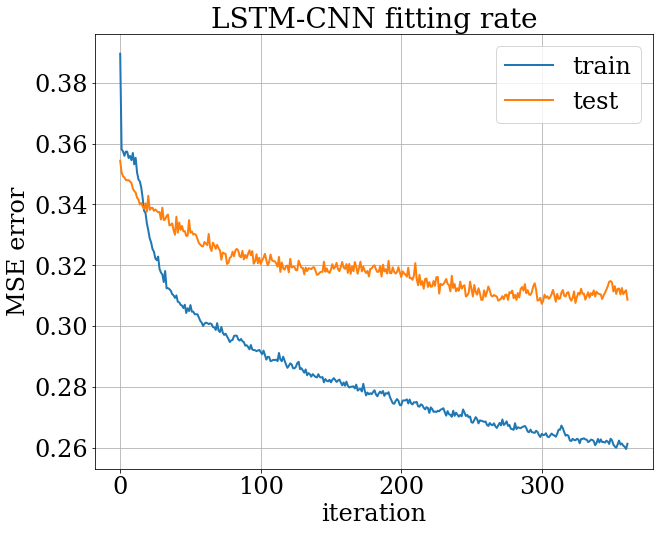
\includegraphics[width=90mm]{conv_graph.png}
\caption{ Basic LSTM CNN model fitting\label{overflow}}
\end{figure}

Along x-axis number of iterations is depicted and along y-axis -  mean square error. Blue curve is used for train loss during whole epoch and orange one - for test loss during validation.

Train error gradually reduces at high rate. That can also be seen in predicted precipitation maps. While in test validation model shows much slower rate and worse predicted results - one of the feature of overfitting. 

\begin{figure}[h] 
\centering
\includegraphics[height=3cm]{train pred.png}
\caption{ Train prediction\label{overflow}}
\end{figure}

\begin{figure}[h] 
\centering
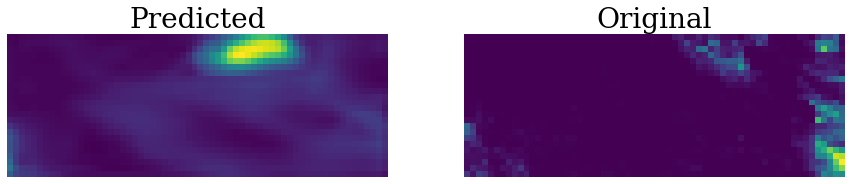
\includegraphics[height=3cm]{test pred.png}
\caption{ Test prediction\label{overflow}}
\end{figure}


Such difference between train and data can be explain with simplicity of basic model when climate changes connections are extremely difficult to build up. However, basic model gives logical and appropriate results. 


\subsection{List of expected figures and tables}
\begin{itemize}
    \item Several figures with predicted climate variables and real ones. Figure is the two same maps from real world with predicted and real heat-maps on the top layer. It will demonstrate quality of prediction.
    \item Table with loss function final errors and F1 or other scores of extreme event classification for at least one model with different hyperparameters and training methods. It will demonstrate which  approach turned out to be the best.
    \item Figure with heat maps predicted by different models. Can be on graph or composed closely together. That will demonstrate influence of classification part of loss function.
    \item Figure of distribution of error on dataset will demonstrate absent of large errors and  number of small errors. Fact that our model will be tuned on extreme prediction.
    
    
\end{itemize}

\pagebreak
\bibliographystyle{plain}
\bibliography{Kornilov2022Winterstorm}

\end{document}